
%Khaled -> Model comparision
\chapter{Modeling}
\label{cha:Modeling}

%----------------------------------------------------------------------------------------
In this part, we have successfully completed the data preparation phase and our sliding windows are ready to use. \newline \newline
Modeling is generally carried out in several iterations. We ran several models using the default parameters and then fine-tuned the parameters. There is not a single model and a single execution which can satisfactorily answer our questions. For this, we tested several models to find the one that best fits our problem.


%----------------------------------------------------------------------------------------
\section{Selecting modeling techniques}

As the first step in modeling, we decided to perform multi-class classification.\newline
Therefore, we have selected Decision Trees and Neural Networks as techniques in order to test its performance and find the most appropriate for our project.

%----------------------------------------------------------------------------------------
\section{Generating a test design}

Before building the model, we used the accuracy results as criteria to compare the performance of the models.\newline \newline
To calculate the accuracy, we separated the dataset into train and test sets, built the model on the train set and estimated its quality on the separate test set. Our test set represents 30\% of the total dataset.\newline \newline
We have also been careful to not shuffling the dataset because we have to keep the right order of the last 10 matches of the sliding window dataset.

%----------------------------------------------------------------------------------------
\section{Building the models}

The aim of this part is to build several models before comparing the results and choosing the one with the best parameters.\newline \newline
Most modeling techniques have a number of parameters that can be adjusted to control the modeling process.
For our project, the Decision Trees can be modified by adjusting the depth of the tree. For Neural Networks, we can change the number of hidden layers, the neurons per layer and other parameters.\newline \newline
Our multi-class classification goal is to predict the final result of a match between two teams. We mean that if the home team wins, the away team wins or draws. It is clear that we have 3 output classes. For this, We used the Decision tree classifier and the Multi-layer Perceptron as a supervised model of Neural network from scikit-learn API. We also built Neural Networks with the TensorFlow framework.


\subsection{Decision Tree Classifier}

A decision tree is a simple classification representation that learns from the data with a set of if-then-else decision rules.\newline \newline
% \cite {DecisionTree: scikit-learn}. 
Using the decision tree algorithm, we start at the root of the tree and divide the data on the feature that results in the largest information gain. We can then repeat this procedure until the leaves are pure.\newline \newline
In our project, we set the depth of the tree at four.\newline
Decision Tree Classifier achieved accuracy of 52.95\% using the first sliding window as the dataset, as shown in the following Figure.

\begin{figure}[h]
\label{fig:DecisionTree}
\begin{center}
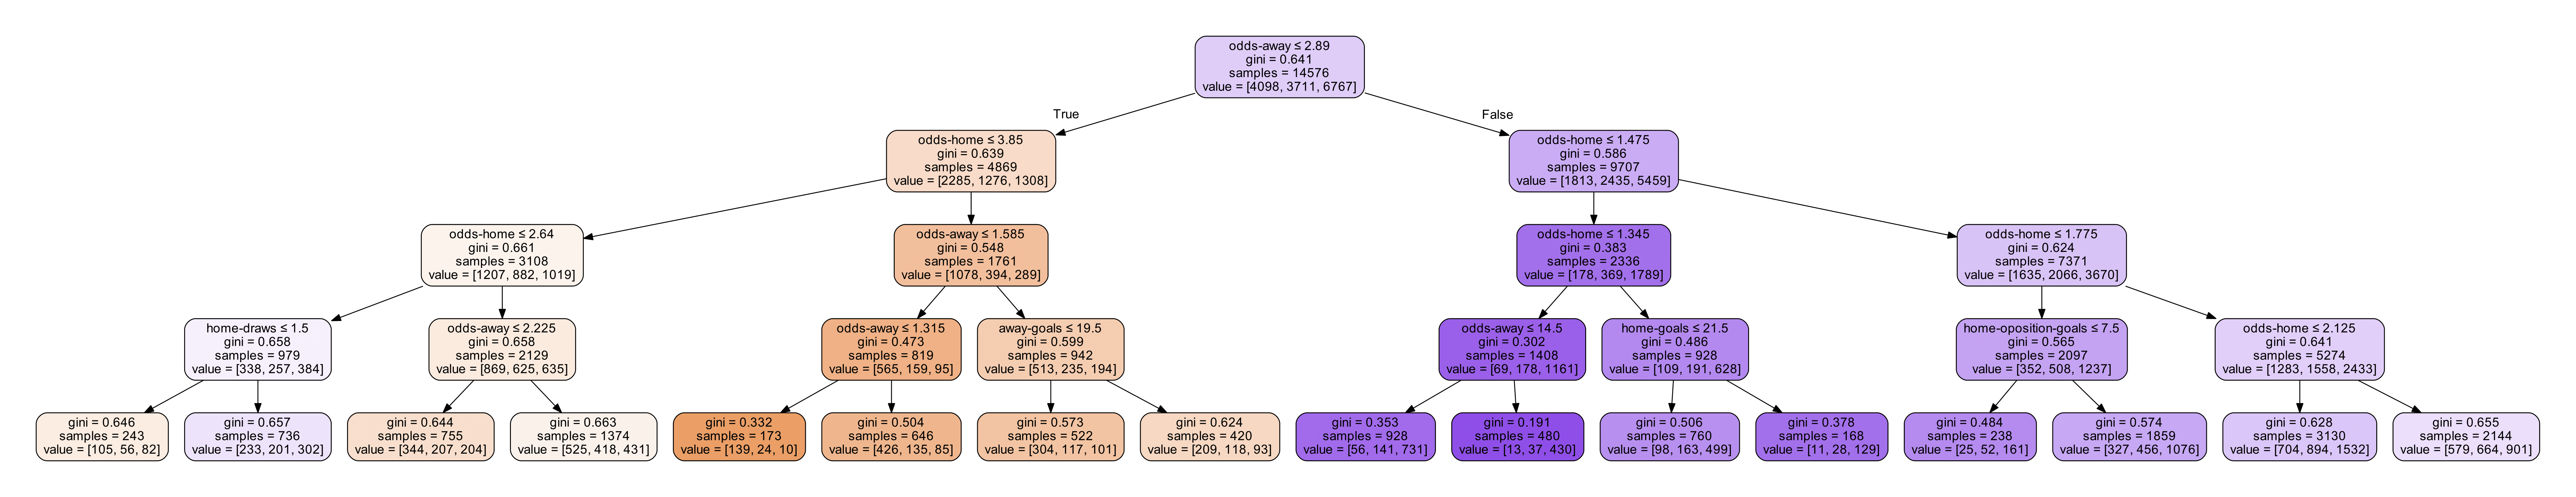
\includegraphics[scale=.07]{DecisionTree}
\end{center}
\caption{Decision Tree (max\_depth=4)}
\end{figure}


\subsection{Multi-layer Perceptron}

Multi-layer Perceptron (MLP) is a supervised learning algorithm consists of three layers: one input layer, one hidden layer, and one output layer. The units in the hidden layer are fully connected to the input layer, and the output layer is fully connected to the hidden layer.\newline \newline %\cite{PythonMachineLearning}
In our MLP Model, we used the first sliding window with 13 features in the input layer, two hidden layers, 52 neurons in the first one and 32 neurons in the second one. For the output layer, we have 3 neurons.\newline \newline  
To be able to solve our problem, we used the sigmoid activation function(logistic) for the hidden layers and the softmax activation function for the output layer. We also used a stochastic gradient descent optimizer as a solver. \newline 
As we see in the following plot, the graph of the cost function indicating that the training algorithm converged after the 90th epoch. \newline

\begin{figure}[h]
\label{fig:MLPcostfunction}
\begin{center}
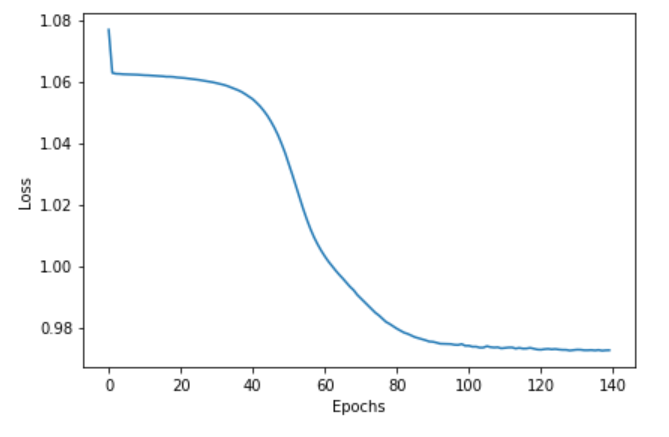
\includegraphics[scale=.7]{MLPcostfunction}
\end{center}
\caption{MLP Cost function}
\end{figure}
The last step is to evaluate the performance of the model by calculating the accuracy of the prediction. We obtained 53.45\% for the training dataset and 52.77\% for the testing dataset.

\subsection{Keras Sequential Model}

To build the model, We used Sequential as a model type. Sequential is the easiest way to create a model in Keras. It allows to build a model layer by layer. Each layer has weights that correspond to the layer that follows it. \newline \newline %\cite{buildingDLModel}
We tested networks with different depths from 1 to 4 hidden layers with a different number of neurons. Our first hidden layer has always more neurons than the input layer. We also have three nodes for the output layer.\newline \newline
We used 'Dense' as the layer type. Dense is a standard layer type that works for most cases. In a dense layer, all the nodes in the previous layer connect to the nodes in the current one.\newline \newline
We used Rectified Linear Activation (ReLU) as the activation function for the hidden layers and softmax for the output layer. Softmax sums the output up to 1 so that the output can be interpreted as probabilities. The model will then make its prediction according to the option which has a higher probability.\newline \newline
The first layer needs an input shape. The input shape specifies the number of rows and columns in the input.\newline
The last layer is the output layer. It has three nodes - one for each option: Home Win, Away Win and Draw, which is for our prediction, as shown in the following line of codes.\newline

$model = tf.keras.Sequential([ \newline
  layers.Dense(13, activation='relu',input\_shape=(train\_X.shape[1],)), \newline
  layers.Dense(16, activation='relu'),\newline
  layers.Dense(8, activation='relu'),\newline
  layers.Dense(3, activation='softmax')\newline
])$ \newline \newline
To compile the model, we chose Adam as an optimizer. The Adam Optimizer adjusts the learning rate throughout the training.\newline
The learning rate determines the speed at which the optimal weights for the model are calculated.\newline\newline
For the loss function, we used $sparse\_categorical\_crossentropy$. It is one of the most common choices for classification. A lower score indicates that the model is performing better.\newline \newline
Weight regularization is another parameter that provides an approach to reduce over-fitting of a deep learning neural network model on training data and to improve the performance of the model on new data.\newline
By default, no regularizer is used in layers. For this, We made some models with the addition of the L2 regularization, which is the sum of the squared weights.\newline \newline
In other models, we have added dropout, which is a regularization technique for neural networks,to avoid over-fitting in neural networks.\newline \newline
We found it interesting to compare the history of the accuracy of several models with different parameters, as shown in the following figure.



\begin{figure}[h]
\label{fig:ModelCompare}
\begin{center}
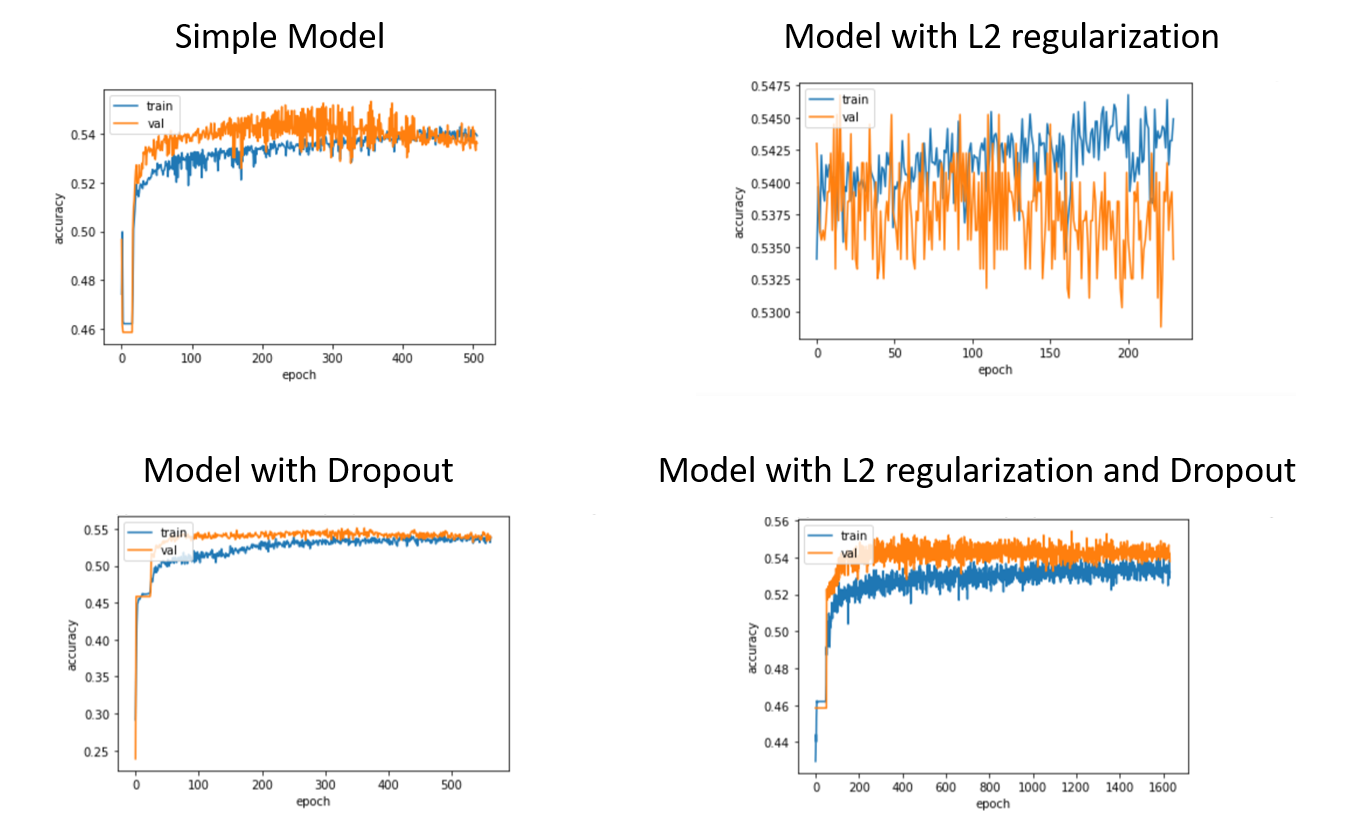
\includegraphics[scale=.6]{ModelCompare}
\end{center}
\caption{Comparison of the history of accuracy models}
\end{figure}


%----------------------------------------------------------------------------------------
\section{Assessing the model}

At this time, we have a set of models, we examined them to determine which one is precise enough to be definitive.\newline \newline
As we explained in building the models part, We created models with different amount of hidden layers and amount of neurons per layer. We also created models with different parameters, as shown in the following figures.\newline \newline


\begin{figure}[h]
\label{fig:colab_nn}
\begin{center}
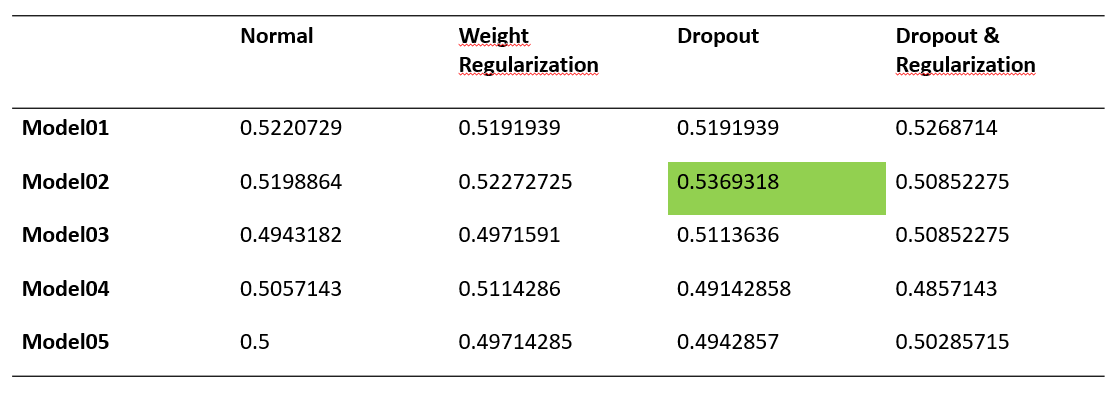
\includegraphics[scale=.7]{colab_nn}
\end{center}
\caption{Comparison between the variation of the sliding windows and parameters}
\end{figure}

\begin{figure}[h]
\label{fig:model3hiddenlayerneurons}
\begin{center}
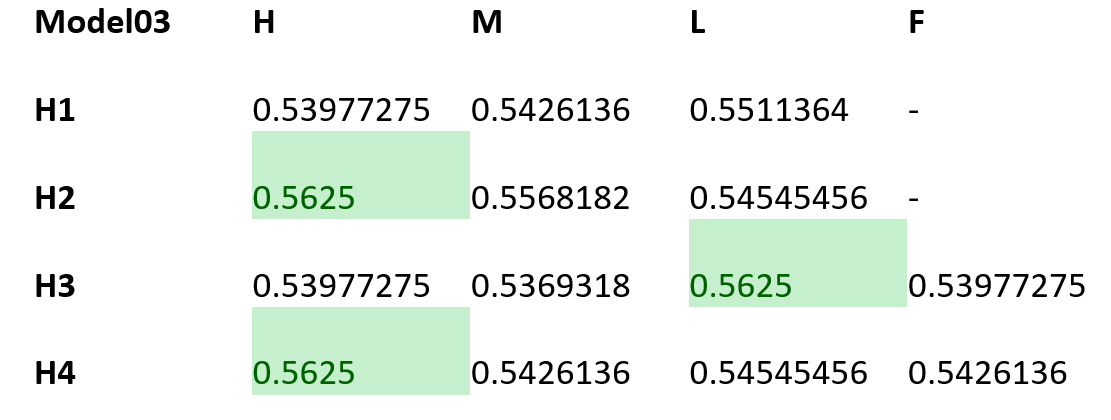
\includegraphics[scale=.7]{model3hiddenlayerneurons}
\end{center}
\caption{Comparison of the models with different amount of hidden layers and amount of neurons per layer}
\end{figure}
According to the evaluation criteria, one of the best simple models uses the third sliding window, which contains 29 features, with two hidden layers with 29 neurons per layer.

%----------------------------------------------------------------------------------------
